\chapter{Generative Graph Models (GGM) and Blasius Realism Framework}
\label{chap:GGM}
\minitoc


\cite{blasius2018towards} presents a general framework that can be used to assess the ability of a \textit{generative graph model (GGM)} to simulate a set of real graphs of interest. They demonstrate their method on a few common GGMs: \textit{Erdos-Renyi (ER)}, \textit{Barabasi-Albert (BA)} preferential attachement graphs, \textit{Chung-Lu} and \textit{Hyperbolic} random graphs. The real graph dataset which they attempt to simulate is a set of 219 real-world networks taken from the \textit{Network Repository} (\url{https://networkrepository.com/}, \cite{rossi2015network}).

Their framework assesses realism of a GGM by using it to produce a dataset of fake graphs. A metric of distinguishability of fake and real datasets based on a select few graph statistics is produced: training a binary SVM classifier of graph \textrightarrow fake/real using the combined fake and real graph datasets as training data, the accuracy of this classifier signifies real/fake distinguishability.

\cite{blasius2018towards} used their framework on a wider range of real-world graphs, but in particular found poor realism of the tested models on the $\approx 100$ strong subset of Facebook social networks that we focus on. We will use the framework to specifically test different types of GIRGs' realism on this tough subset, with the hope that they will do better than the previous best models - Chung-Lu and Hyperbolic. We also think that restricting to this one subset of what should be similar types of real-world graphs will allow clearer differentiation between different GGMs.

% Hence realism is evaluated on the chosen few graph statistics (e.g. mean node degree in a graph, or graph diameter), and at a higher collection level, which helps to 

% assesses realism of the generative models by fitting them to the real graphs so as to produce a collection of similar fake graphs, and then determing the similarity/distinguishability of the two collections of real graphs and fake graphs. This comparison itself is done on the basis of a select few graph statistics - like mean node degree or graph diameter, so realism is ability of the generative model to produce graphs with a sequence of statistics indisinguishable

% Erdos-Renyi (ER), Barabasi-Albert (BA) preferential attachement graphs, Chung-Lu and Hyperbolic Random graphs.
% They are compared on the basis of their ability to simulate real graphs of interest, such as social networks, citation networks, and biological networks, which are known to have power law node degree distributions.


\section{GGM and Framework Mathematical Outline}
A graph $G = (V,E)$ is said to be randomly generated from a GGM $\cG$, written $G \sim \cG$. Most of our GGMs are simple and can be described by a small number of parameters. For example for the Erdos-Renyi GGM, $G \sim \cG_{ER}(n, p)$ means that there are $n$ nodes: $V=[n]$, and each potential edge $(u,v)$ exists iid with probability $p$, i.e. $p(u \sim v) = p$.

\subsection{Fitting a GGM to a particular real graph instance}
\label{sec:fitting_GGM}
\q{Fitting} a GGM to a real graph $G$ means finding the most plausible $\hat{\theta}$ in the hypothetical world where $G$ was produced via $G \sim \cG(\hat{\theta})$. Hence for our ER GGM example, choosing $\hat{n} = |V|$ is a no-brainer, and $\hat{p} = |E| / \binom{n}{2}$ follows by fitting the expected number of edges.

Fitting $\hat{\theta}$ can also be done by likelihood estimation. This is tractable for the Erdos-Renyi GGM, by solving $\argmin_p \sum_{u \neq v} e_{uv} \log(p) + (1 - e_{uv}) \log( 1 - p)$, where $e_{uv}$ is the edge indicator function, which gives the same $\hat{p}$ as above. For GIRGs however, this would be intractable: for example we cannot even easily integrate over all possible point locations in the geometric space:

\begin{equation*}
    p(G | \alpha, \vec{w}, d) = \int_{\vec{x}_1 \in [0,1]^d} \cdots \int_{\vec{x}_n \in [0,1]^d} p(G | \alpha, (\vec{x}_i)_{i=1}^n) \prod_{i=1}^n p(\vec{x}_i)
\end{equation*}

Instead we can use a heuristic method based on \textit{Approximate Bayesian Computation (ABC)}. We seek the parameter $\hat{\theta}$ that minimises the expected distance $ \E[\delta(G, G' \sim \cG(\theta))]$ for some distance metric $\delta$. This basically means that the GGM parametrised by $\hat{\theta}$ successfully generates graphs $G'$ that look similar to our given graph $G$.
For $\delta$ to be effective, ideally it would be something like $(f(G) - f(G'))^2$, for $f$ a sufficient statistic of $\theta$. In practice this looks like an algorithm where we repeatedly sample $\theta$ from a prior; use it to generate $G'$; see if $f(G') \approxeq f(G)$, and if so keep $\theta$ as a candidate for $\hat{\theta}$.

\subsection{Plausibility of Fitted GGMs}

Similarly to the use of a statistic $f$ of real and generated graphs as a proxy for fitting $\hat{\theta}$, we can also use other high level statistics $\fclass$ to evaluate the plausibility of a fitted GGM as to whether it could have produced the real graph $G$. We will later use these as the input features to the real/fake binary classifier, hence the notation.

Having fit $\hat{\theta}$ of the GGM, we can then sample graphs $G' \sim \cG(\hat{\theta})$ which are hypothetically similar to $G$. We can only hope for similarity on the global level. Even in the best case scenario where both $G, G' \sim \cG(\hat{\theta})$, there is no local identification of nodes and edges, e.g. we cannot expect  $e \in E \iff e \in E'$ - see \cref{chap:graph_kernels} for more on graph similarity.

For example in the Erdos-Renyi exact fit case, in the best case scenario we have $G \sim \cG_{ER}(n, p^*)$ and $G' \sim \cG_{ER}(n, \hat{p} = p^* + \epsilon)$. Although there will be some small estimation error $\epsilon$ in the fit parameter (which may be biased to be non-zero if e.g. $G$ randomly has $|E|$ differing from $p^* {n \choose 2}$), we've explicitly fit for the high level statistic of the number of edges, s.t. $|E| = \E[|E'|] = \hat{p} \binom{n}{2}$, and $|E'| \approxeq |E|$ with some small variance. For other (not fit) high level statistics $\fclass$ like the effective diameter of the graph, their expected value will be close to that of $G$, $E_{G' \sim \cG(\hat{\theta})}[\fclass(G')] \approxeq \fclass(G)$, and likewise concentrated with small variance s.t. $\fclass(G') \approxeq \fclass(G)$.


Furthermore if we were to generate a whole list of graphs $G'_1, \dots, G'_m$ from $\cG(\hat{\theta})$, assuming the matching GGM hypothesis, we would not expect $G$ to stand out from the crowd. Essentially the random variable $\fclass(G'(G))$ should follow a distribution with $\fclass(G)$ not too far from the mean/median, in an empirical p-value sense.


\subsection{Fitted GGMs as candidates for real graphs - Blasius}
\label{sec:ggm_blasius_framework}
\cite{blasius2018towards} takes this method one step further. They are essentially evaluating the hypothesis that the set of real graphs $G_1, ..., G_k$ are generated from a particular GGM $\cG$, but with differing parameters: $G_1 \sim \cG(\theta^*_1), ..., G_k \sim \cG(\theta^*_k)$. Perhaps $\theta^*_i$ come from some prior distribution $p(\theta)$.

They again fit individual $\hat{\theta}_i$ with which to generate one $G'_i \sim \cG(\hat{\theta}_i)$ per real graph $G_i$. This way instead of, for each real graph, comparing multiple $G'_{ij}$ to $G_i$ and averaging, they can compare the set of graphs $\{G_i\}_{i=1}^k$ to $\{G'_i\}_{i=1}^k$. Graph comparison is done by comparing a wide number of statistics/metrics computed for each graph. These are input as a whole feature vector $\vec{f}^\mathrm{class}(G)$ to an SVM classifier, which is trained to classify membership of the real or generated dataset. These features are statistics such as the number of nodes, mean node degree, mean node closness centrality, graph diameter and so on.


Performing this classification task over the whole dataset of graphs allows for a GGM realism evaluation without needing to have the additional computation of generating multiple $G'_{ij}$ for each real graph $G_i$, which would have given a more detailed graphwise GGM realism metric. There is an added benefit of helping to cover for GGM parameter fitting inaccuracy. If $\hat{\theta}_i = \theta^*_i + \epsilon_i$, it may still be possible to distinguish $G_i$ from $\{G'_{ij}\}_{i=1}^m$ due to the $\epsilon_i$ fitting error. If instead we compare the set $\{\theta^*_i\}_{i=1}^k$ to $\{\hat{\theta}_i\}_{i=1}^k$, Now each $\hat{\theta}_i \neq \theta^*_i$, but still well fits into the distribution of $\{\theta^*_i\}_{i=1}^k \sim p(\theta)$. Finally having one $G'_i$ per real graph $G_i$ also simplifies the binary classification task by having a balanced dataset.

% We suggested in the previous section that multiple $G'_{ij}$ could be generated per real graph $G_i$ - this would reduce the variance of the whole process. This is also necessary to be able to train a classifier on an individual real graph basis, as you cannot do binary classification on just a pair of feature vectors $\vec{f}^\mathrm{class}(G_i)$ and $\vec{f}^\mathrm{class}(G'_i)$. Blasius instead aggregates the classification over the whole dataset of real graphs, allowing sufficient datapoints to train a classifier while reducing the overall necessary computation ($k$ generated graphs produced instead of $km$).


% This gives us a mirrored real/fake graph features dataset: $\{\vec{\fclass}_i (G)  = \vec{\fclass}(G_i)$ for feature vector function $\vec{\fclass}$, against $\vec{\fclass}_i$.
The output of the Blasius framework, for a given GGM and classification feature vector $\fclass$, is a real/fake accuracy percentage. If it were really the case that the input real-graphs were generated from $G_i \sim \cG(\theta^*_i)$ of the same GGM $\cG$ as the fitted fake graphs, the SVM should be able to acheive only close to $50\%$ accuracy, as real and fake $\fclass$ should be hard to tell apart. Higher accuracies denote distinguishability of real from fake - occuring if instead $G_i \sim \tilde{\cG}(\phi^*_i)$ for some alternative GGM $\tilde{\cG}$.


% Contextually, GIRGs are compared with other generative graph models: Erdos-Renyi (ER), Barabasi-Albert (BA) preferential attachement graphs, Chung-Lu and hyperbolic graphs.
% In \cite{blasius2022efficiently}


% In fact, in the best case, actually $G \sim \cG(\theta^*)$, so our parameter estimate is $\hat{\theta} = \theta^* + \epsilon$. Here $\epsilon$ is a random noise in our ability to fit $\theta$, hopefully small and with mean zero. 

% Then for any statistic $f$, we could consider the randomness $f(G) \sim F_1$, and $f(G') \sim F_2$. Due to the $\epsilon$ error in $\theta$ estimation, $F_2| \hat{\theta}(G) \nsim F_1$, but we would hope that $f(G)$ would still be reasonably within distribution, and less strongly (???) that $F_2 \sim \approxeq F_1$ not too far off, rather likely a higher variance but otherwise similar distribution.

% % To give a concrete example, say that $F|\theta \sim N(\theta, 1)$, and that $\theta^* = 0$. Then $F_1 \sim N(0, 1)$, and $F_2 | \epsilon  \sim N(\epsilon, 1)$. Assume perverseley that $F_1 | \epsilon \sim N(-\epsilon, 1)$, although perhaps something like $N(\epsilon / 2, 1)$ is more likely. 

% Hence plausibly sampling $G_1, ..., G_k \sim \cG(\theta^*)$, fitting $\hat{\theta}_i(G_i)$ and further sampling $G_i' \sim \cG(\theta^*)$, we expect that $f_i \sim F_1$ would be hard to separate from $f_i' \sim F_2$ with a classifier.



% $p(\alpha | G, \vec{w}) = \int_{\vec{x}}  \frac{p(G | \alpha, \vec{w}, \vec{w}) p(\alpha)


\section{Fitting GIRG GGM to a real graph}
The GGM parameters of the GIRG model $\cG_{\GIRG}(\theta)$ are $\theta = (n, d, c, \alpha, \tau)$. For the Blasius framework we need to fit $\hat{\theta}$ to a given real graph $G$, as the best estimate for the parameters that would have generated $G \sim \cG_{\GIRG}(\theta)$. The problem of fitting dimension $d$ is a tricky one that we touch on briefly in \cref{chap:diff_maps}. We also attempted to use \textit{graph fractal dimension} to infer $d$ without success. We instead avoid the problem by treating 1d, 2d, 3d etc. GIRGs as separate GGMs, to be individually fitted and inter-compared.

\subsection{Fitting number of nodes $n$}

We follow \cite{blasius2018towards} which first preprocesses the graph $G$ by shrinking it to its largest connected component, $G \gets \shrinktogcc(G)$
before fitting $\cG$ to it. Then $n$ is just the number of remaining nodes.


% This is not because the GIRG model always generates connected graphs, which is not true. 

Blasius' rational is that where some real graphs in our dataset have disconnected subgraphs, this may be due to them being a concatenation of a few distinctly generated subraphs, hence a GGM should be fit just to one subgraph (the largest - the rest are discarded for potentially being too small). All of our GGMs are capable of producing a bunch of disconnected subgraphs, however this is most likely to occur in our geometric GGMs which exhibit clustering; GIRGs do at least whp produce a unique giant component - one with a linear number of nodes. Hence for a fair comparison $d(G, G')$, we also need to post-process the GGM generated $G' \gets \shrinktogcc(G')$. 

Blasius's only geometric model is Hyperbolic Random Graphs, for which they use a fitting algorithm that actually estimates a higher number of nodes $n > |V|$ in order to approximately have the largest connected component of $G' \sim \cG$ be of size $|V|$.
We don't do this for our GIRGs however, as we find this algorithm prone to error, and unnecessary, at least for the socfb Facebook graphs - see \cref{tab:blasius_HRG_n_fitting_renunciation}. We accept instead that our GGMs may end up with slightly fewer nodes than the real graphs, and hope that this doesn't affect the SVM classification too much.


% Hence if any real graph had multiple giant components (say e.g. $V = A \sqcup B \sqcup (...)$ with $|A| = n/2,\; |B| = n/3$), then we would not expect any of our GGMs to fit well to the whole graph.

Restricting graphs to a connected component also has the added benefit of making some graph statistics more meaningful/sensical - for instance diameter and path lengths.

% This explains why Blasius even further post-processes the GGM generated fake graphs to also restrict to their largest connected component.
% Blasius goes as far as to, for the hyperbolic GGM, using a fitting algorithm that actually estimates a higher number of nodes $n > |V|$ in order to approximately have the largest connected component of $G' \sim \cG$ be of size $|V|$. We don't do this for our GIRGs however, as we find this algorithm prone to error, and unnecessary, at least for the socfb Facebook graphs.

\begin{table}[]
    \centering
    \begin{tabular}{|c|c|c|}
    \hline
    \textbf{graph name} & \textbf{GGM} & \textbf{nodes} \\ \hline
    socfb-American75 & real-world & 6370 \\ \hline
    socfb-American75 & 1d-girg & 6370 \\ \hline
    socfb-American75 & 2d-girg & 6370 \\ \hline
    socfb-American75 & 3d-girg & 6370 \\ \hline
    socfb-American75 & ER & 6370 \\ \hline
    socfb-American75 & chung-lu & \textcolor{cyan}{6279} \\ \hline
    socfb-American75 & hyperbolic & \textcolor{orange}{6583} \\ \hline
    socfb-Amherst41 & real-world & 2235 \\ \hline
    socfb-Amherst41 & 1d-girg & 2235 \\ \hline
    socfb-Amherst41 & 2d-girg & 2235 \\ \hline
    socfb-Amherst41 & 3d-girg & 2235 \\ \hline
    socfb-Amherst41 & ER & 2235 \\ \hline
    socfb-Amherst41 & chung-lu & \textcolor{cyan}{2221} \\ \hline
    socfb-Amherst41 & hyperbolic & \textcolor{orange}{2282} \\ \hline
    % \begin{comment}
    % socfb-Auburn71 & real-world & 18448 \\ \hline
    % socfb-Auburn71 & 1d-girg & 18448 \\ \hline
    % socfb-Auburn71 & 2d-girg & 18448 \\ \hline
    % socfb-Auburn71 & 3d-girg & 18448 \\ \hline
    % socfb-Auburn71 & ER & 18448 \\ \hline
    % socfb-Auburn71 & chung-lu & \textcolor{cyan}{18325} \\ \hline
    % socfb-Auburn71 & hyperbolic & \textcolor{orange}{18787} \\ \hline
    % socfb-BC17 & real-world & 11498 \\ \hline
    % socfb-BC17 & 1d-girg & 11498 \\ \hline
    % socfb-BC17 & 2d-girg & 11498 \\ \hline
    % socfb-BC17 & 3d-girg & 11498 \\ \hline
    % socfb-BC17 & ER & 11498 \\ \hline
    % socfb-BC17 & chung-lu & \textcolor{cyan}{11393} \\ \hline
    % socfb-BC17 & hyperbolic & \textcolor{orange}{11824} \\ \hline
    % \end{comment}
    ... & ... & ... \\ \hline
    bio-diseasome & real-world & 516 \\ \hline
    bio-diseasome & 1d-girg & \textcolor{cyan}{258} \\ \hline
    bio-diseasome & 2d-girg & \textcolor{cyan}{491} \\ \hline
    bio-diseasome & 3d-girg & \textcolor{cyan}{496} \\ \hline
    bio-diseasome & ER & \textcolor{cyan}{512} \\ \hline
    bio-diseasome & chung-lu & \textcolor{cyan}{459} \\ \hline
    bio-diseasome & hyperbolic & \textcolor{cyan}{125} \\ \hline
    \end{tabular}
    \caption{
    % For the socfb Facebook graphs, we see that the chung-lu model consistently has a very small number of nodes disconnected from the giant component, hence ending up with fewer nodes than the input (shrunk to GCC) real graph. 
    For the socfb Facebook graphs, the hyperbolic model consistently has a few more nodes than the input real graph due to its fitting algorithm not quite working perfectly (and stochasticity).
    On other real graphs there can be larger discrepancies, especially for smaller extra sparse graphs.
    Numbers of nodes in the output (shrunk to GCC) graph are colored \textcolor{cyan}{cyan} if less than the real-world graph, and \textcolor{orange}{orange} if more (only possible in hyperbolic case).
    }
    \label{tab:blasius_HRG_n_fitting_renunciation}
\end{table}
    



Note that GIRGs might still do the best job, compared to other non geometric GGMs, of fitting multiple large components, as they have the property of containing sublinear separators. Essentially if you divide the torus with a hyperplane (or divide out a sub-cube), $\chi = \chi_A \sqcup \chi_B$, to produce disjoint node subsets $V_A \sqcup V_B = V$ and their induced subgraphs $G_A, G_B$, then whp $G_A$ has sublinear of $|V_A|$ edges to $G_B$ (despite having linear number of edges within itself). Also interestingly $G_A$ is stochastically still a (smaller) GIRG, just one with a non-toroidal geometry.





% For example when fitting the Chung Lu Model this makes a lot of sense
% However it should be noted that GIRGs don't always produce connected graphs if the probabilities are scaled down. Furthermore they 
% GIRGs do have the property that the subraph from restricting to a smaller subsection of the Torus stochastically is still a GIRG (with a non toroidal geometry), and may even be disconnected from the rest of the graph (Note that if present, most larger disconnected subgraphs within a GIRG are usually also "geometric subgraphs").



\subsection{Fitting power law distribution exponent $\tau$ for node weight sampling}
We fit $\tau$ to the tail of the \textit{degree distribution} of $G$, using the python package $\PLP$. Having this fit parameter enables subsequent generation of new weight sequences $w_u \sim \powerlaw(\tau)$ for sampling new GIRGs $G' \sim \cG_{\GIRG}(\tau,...)$.

\paragraph{The degree distribution} of the graph $G$ is defined as $dd(x) := \frac{|\{v \in V: d(v) = x\}|}{|V|}$, i.e. the fraction of nodes with degree $x$. For graphs generated by the GIRG model, we noted that the geometry marginalisation property means that $E[d_u] \propto w_u$. Hence if node weights are distributed following $\powerlaw(\tau)$, we expect to see the tail of the degree distribution, $dd(x)$ as $x \to n$ to look like a discrete power law distribution $dd(x) \propto x^{-\tau}$.

\paragraph{Sketch of why GIRG power law weights \textrightarrow\ power law degree distribution}  
% that $dd(x) \approxeq P(d_u = x) \approxeq P(w_u = x) \propto x^{-\tau}$.
By treating node degrees as roughly iid, $dd(x) \stackrel{n \to \infty}{\to} P(d_u = x)$.
For a fixed weight $w_u$, node degree $d_u$ closely follows a binomial distribution $\binomial(n-1, \Theta(w_u / n))$, so we'd like to calculate 
\begin{equation}
    P(d_u = x) = \int P(d_u = x | w_u = w) \Theta(w^{-\tau}) \,dw
\end{equation}
For sufficiently large $x$ (in the tail of the decaying distribution of $dd(x)$), the binomial distribution of mean and variance $w$ is sharply peaked around its mean: if $(x-w) > w^{1/2 + \epsilon}$ then $P(d_u = x | w_u = w) \approx 0$. 
So essentially all the probability mass is on the region $[x - x^{1/2 + \epsilon}, x + x^{1/2 + \epsilon}]$, on which $\Theta(w^{-\tau}) \approx \Theta(x^{-\tau})$ (doesn't change much at all) as e.g. $(x - x^{1/2 + \epsilon})^{-\tau} = (x[1 - x^{-1/2 + \epsilon}])^{-\tau} \approxeq x^{-\tau}$ for large $x$.
Hence $dd(x) \stackrel{n \to \infty}{\to} \Theta(x^{-\tau})$ for large $x$.


% This means that for sufficiently large $x$, we can focus on just the subsection of the integral $\int_{x-x^{1/2 + \epsilon}}^{x + x^{1/2 + \epsilon}}$.
% In this subsection, $\Theta(w^{-\tau}) \approxeq \Theta(x^{-\tau})$, and we can approximate the binomial distribution as a gaussian with mean and variance $w$. This has pdf $\frac{1}{\sqrt{2 \pi w}} e^{-(x-w)^2/2w}$ which we can approximate as $\frac{1}{\sqrt{2 \pi x}} e^{-(w-x)^2/2x}$.

% Finally we evaluate
% \begin{equation}
% \int_{x-x^{1/2 + \epsilon}}^{x + x^{1/2 + \epsilon}} \frac{1}{\sqrt{2 \pi x}} e^{-(w-x)^2/2x} \; \Theta(x^{-\tau}) dw = \Theta(x^{-\tau})
% \end{equation}
% to get a discrete power law distribution for $dd(x)$

% Instead we simplify the binomial distribution (which has mean and variance $\Theta(w_u)$); we just treat $d_u$ as a distribution peaked sharply around its mean $\Theta(w_u)$, e.g. a delta function $\delta(x - \Theta(w_u))$, to derive that $\P(d_u = x) = \Theta(x^{-\tau})$.

% and so $P(d_u = x) \approxeq \int \Theta(w^{-\tau}) \binomial(n-1, \Theta(w / n))(x) dw$, i.e. $\int \Theta(w^{-\tau}) P(d_u = x | w_u = w) dw$. Th

% For large $x$, only $w$ s.t. $w = \Theta(x)$ contribute non-negligibly to the integral

% A brief sketch of why this occurs:

% We saw previously that regardless of the GIRG geometry, $P(u \sim v | w_u, w_v) = \Theta(\frac{w_u w_v}{n})$.

% More specifically, this gives that $P(u \sim v | w_u) = p_u = \Theta(\frac{w_u}{n})$, such that the degree $d_u \sim Bin(n-1, p_u)$.
% WHP, as $n \to \infty$, $\forall u,\; w_u = o(n)$ s.t. $p_u = o(1)$ and so $d_u$ converge in distribution to $Poisson(\Theta(w_u))$.
% % (I get the $p_u, w_u$ bit, but not the $d_u$?).
% This means that $\E[d_u] = \Theta(w_u)$, and so $\E[dd(x)] = \E[ \frac{ \sum_u 1_{d_u = x}}{n}] = \E[d_u = x]$. This we can calculate as $\int_w P(w_u = w) P(d_u = x | w_u = w)dw = \int_w w^{-\tau} \PP(\Poisson(\Theta(w)) = x) dw$. It's essentially the inner product (integral of product) of two probability distributions, the first is $w^{-\tau}$, the second is a Gaussian looking like function with mean and variance $\Theta(w)$, and hence to first order the integral is $\Theta(w^{-\tau})$ (e.g. if you changed the gaussian integral to have the same mean $w$ but variance squeezed $\sigma^2 \to 1$ as to be like a delta function). It follows that for large $x$, $\E[dd(x)] = \Theta(x^{-\tau})$.

\paragraph{powerlaw package fitting}
Therefore if $G$ is a $\tau$ exponent power law weighted GIRG , we expect its degree distribution $dd(x)$ for large degrees $x$ to look like $dd(x) \propto x^{-\tau}$. Hence we can fit $\tau$ on this tail. \PLP does this by simultaneously finding a lower bound $x_{\min}$ for where in the tail the power law behaviour starts, and fitting $\tau$ to the region $x > x_{\min}$ using maximum likelihood estimation\footnote{A visually much more compelling method of fitting the power law degree distribution tail is to plot the empirical degree distribution on a log-log scale, and literally draw a line of best fit on the heavy tail - $w^{-\tau}$ will look like a straight line with gradient $-\tau$. In fact one minus the empirical cdf is even better as it looks like $w^{1-\tau}$, so a similar log-log linear fit works to find $\tau$, and the plotted points are more robust to noise}. The optimal $x_{\min}$ is chosen to minimise the Kolmogorov-Smirnov distance between the power law fit and the region's emprirical degree distribution.

Having fit $\tau$, we can then sample weights $w_u \sim \powerlaw(\tau)$.

% \subsubsection{Power Law Distribution}
% A power law distribution $x \sim \powerlaw(\tau)$ simply has pdf $p(x) \propto x^{-\tau}$ with support $x \in [1, \infty]$, i.e. default $x_{\min} = 1$.

\subsection{Power Law weight alternative: weight copying}
Generating weights $w_u \stackrel{iid}{\sim} \powerlaw(\tau)$ is fine as a model prior, however it's not a perfect fit to real-world data. This is particularly true as real graph degrees generally only follow a power law for large degrees; they might be better modelled by a GIRG with node weights with a power law tail (e.g. upper quartile of weights) and a different distribution for the rest of the weights. Most obviously, instead of having peak number of nodes with weight $w_u = x_{\min}$, the weight distribution might follow a more natural curve like in \cref{fig:natural_weight_distribution}.


\begin{figure}
    \centering
    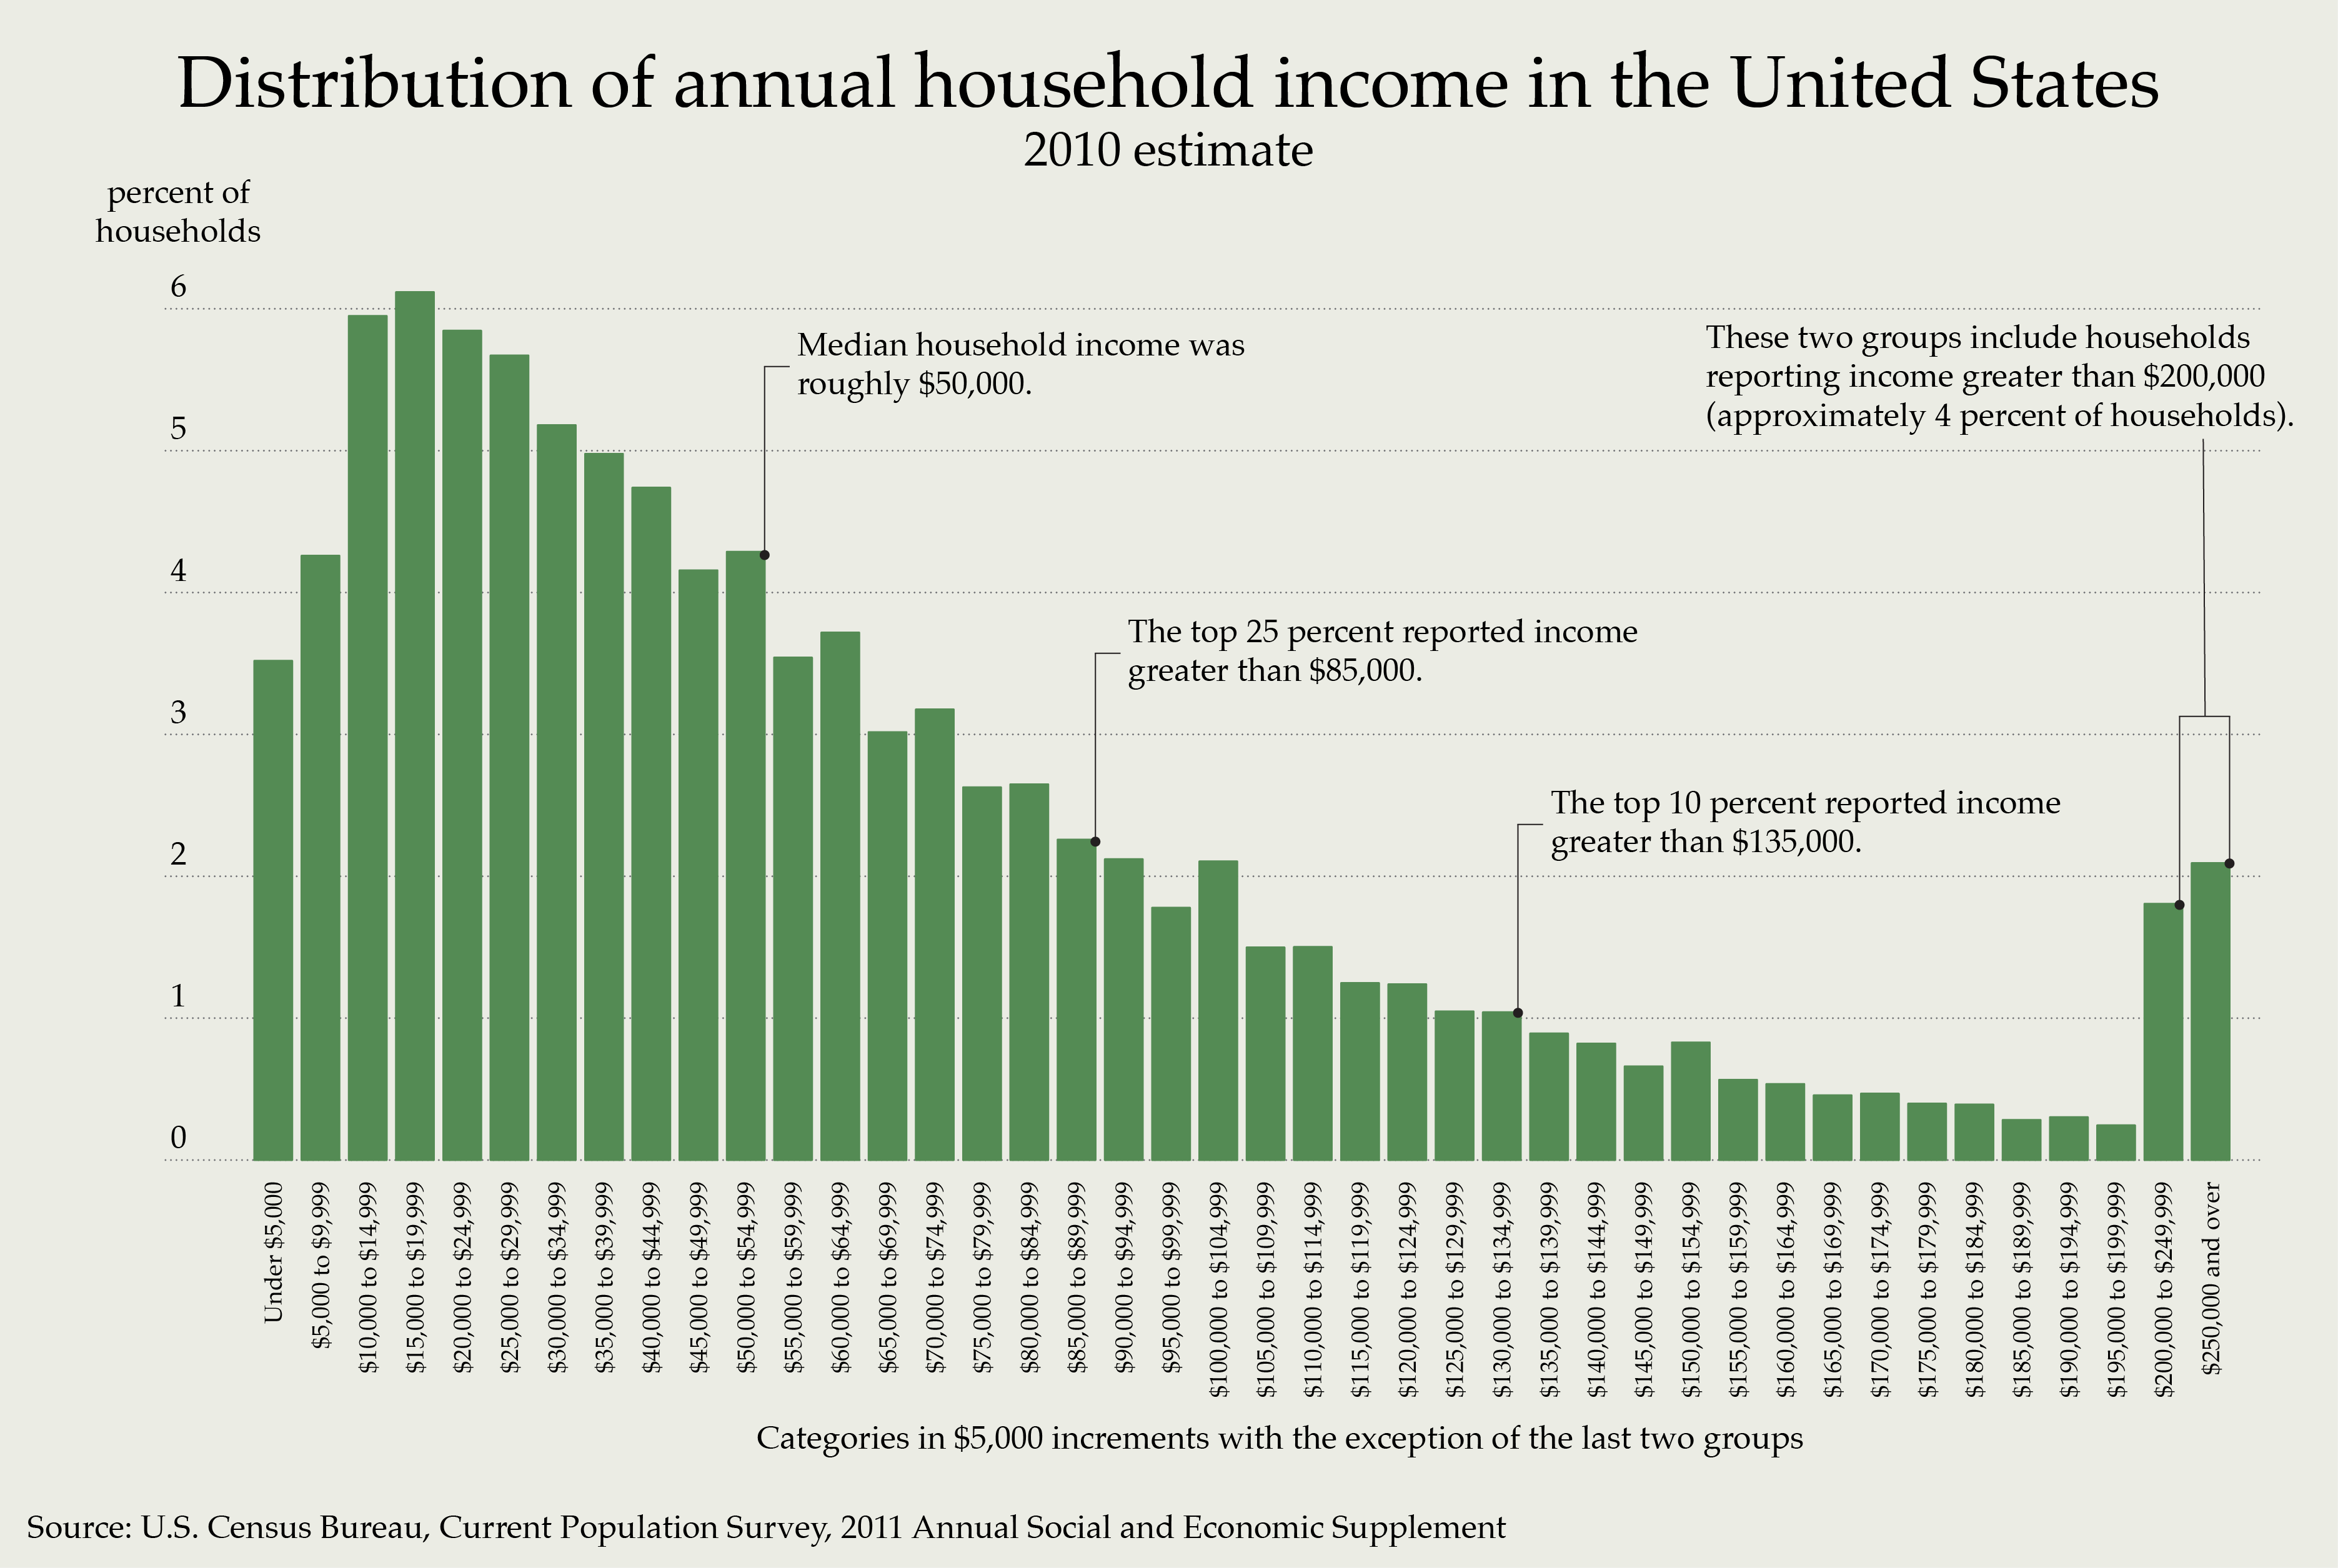
\includegraphics[width=\textwidth]{./figures/Distribution_of_Annual_Household_Income_in_the_United_States_2010.png}
    \caption{Example of a more natural weight distribution with a power law tail but not for smaller weights.}
    \label{fig:natural_weight_distribution}
\end{figure}

% This is particularly true as power laws 
% A sequence of weights with a constant q-tile of largest weights fitting into $\tau$ powerlaw tramlines fits the general GIRG formulation, but could still look quite different based on the distribution of the smaller weights.

An easy improvement to better fit a specific real graph is to take the sequence of node degrees as weights
\footnote{these are now all positive integers $\geq 1$ as opposed to real numbers $\geq x_{\min}$, since in the largest connected componenet, minimum degree is 1}. Copying degrees as weights makes sense due to the Chung-Lu like property of having $E[d_u] \propto w_u$, whose correct scaling can be made correct by fitting $c$ as detailed in the next section. 
% For the GIRG model however there is the added complication of node locations, whereby a node might have a higher degree than expected for its weight $w_u$, by fortune of having many geometrically close nearby nodes $\vec{x}_v$.
% This would clearly have better classification performance than power law generating weights.
For the classification comparison framework, Blasius actually uses weight copying for fitting the Chung-Lu GGM, but not for the hyperbolic GGM (which is odd). This doesn't make a fair / like for like comparison, so we cover all bases by having both weight copied and power law fit GIRGs, as well as adding in a power law fit Chung-Lu. ER and BA GGMs are still just fit on the courser metric of overall graph average degree, as they have little ability to replicate a power law degree distribution.

Comparing weight copied Chung-Lu with weight copied GIRGs was additionally interesting for harder feature sets where other GGMs struggled to get below 98\% classification accuracy - having such high constrained numbers makes it harder to compare meaningfully between GGMs (drawing conclusions from 98\% vs 99\% is tough)

% Comparing weight copied Chung-Lu with weight copied GIRGs was additionally interesting as their classification from real graphs was harder and hence more informative (trying to compare a 97\% vs 99\% classification accuracy is less meaningful than a 80\% vs 90\%).

% (QUESTION: does the GIRG formulation actually guarantee that as n -> infinity you couldn't tell the difference? I don't think so. E.g. if 1/4 of nodes had w=1, 1/4 had w=10 and 1/2 were power law above 10 distributed.)


\begin{comment}
Integrating $\int_w w^{-\tau} \PP(\Poisson(\Theta(w)) = x) dw$ gives $\E[dd(x)] = \Theta(x^{-\tau})$, for large $x$, dropping smaller order terms.


If instead, independently, each $d_u = \E[\Poisson(\Theta(w_u))] = \Theta(w_u)$, then we would sort of be able to say that the degree distribution follows a $\tau$ exponentiated power law distribution.
We would argue that independently, $P(d_u=m) \approxeq \Theta( \int_{m-1/2}^{m+1/2} w^{-\tau}) = \Theta(m^{-\tau})$, and hence that $dd(m) \sim \frac{Bin(n, m^{-\tau})}{n} \to N(m^{-\tau}, \frac{m^{-\tau}(1- m^{-\tau})}{n}) \approxeq m^{-\tau}$.

Ok so now if $d_u \sim \Poisson(\Theta(w_u))$, can we then derive $\PP(d_u = d)$? $\PP(d_u = d) = \int_W \PP(d_u = d | w_u = w) p(w) dw$. For large $w$, we approximate $\Poisson(\Theta(w_u)) \approxeq N(\Theta(w_u), \Theta(w_u))$. Hence we get $\PP(d_u = d) \propto \int_W \exp(-\frac{(w-d)^2}{2w}) w^{-\tau} dw$. We approximate this integral to be dominated by the interval $w \in [d - k\sqrt{d}, d + k\sqrt{d}]$ for sufficiently large $k$.

So we get $\PP(d_u = d) \propto \int_{d - k\sqrt{d}}^{d + k\sqrt{d}} \exp(-\frac{(w-d)^2}{2w}) w^{-\tau} dw \approxeq \int_{d - k\sqrt{d}}^{d + k\sqrt{d}} \exp(-\frac{(w-d)^2}{2d}) w^{-\tau} dw$. 

Substitute in $x = w - d$ to get $\int_{-k \sqrt{d}}^{k \sqrt{d}} (d + x)^{-\tau} e^{-x^2/2d}dx$.

Then using $(d + x)^{-\tau} = d^{-\tau} (1 + \frac{x}{d})^{-\tau} \approxeq d^{-\tau} (1 - \frac{\tau x}{d} + \frac{\tau(\tau+1)}{2} \frac{x^2}{d^2})$ for $x \in [-k \sqrt{d}, k \sqrt{d}]$, we get $\int_{-k \sqrt{d}}^{k \sqrt{d}} (d + x)^{-\tau} e^{-x^2/2d}dx \approxeq d^{-\tau} \int_{-k \sqrt{d}}^{k \sqrt{d}} (1 - \frac{\tau x}{d} + \frac{\tau(\tau+1)}{2} \frac{x^2}{d^2}) e^{-x^2/2d}dx$.

Finally we can use the results on the pdf of a normal distribution integrating to $1$; the mean integrating to $0$, and the variance integrating to $\sigma^2$, to get that $\PP(d_u = d) \propto d^{-\tau} (1 + \frac{\tau(\tau + 1)}{2} d^{-2} d) = d^{-\tau} 1 + \frac{\tau(\tau + 1)}{2} d^{-(\tau + 1)}$. This formula is essentially a weighted average between two different power law distributions. As $d \to \infty$ it will actually be correct, and be dominated by the larger $d^{-\tau}$ term. However for not so large $d$, it will be more a mix, and so the "perceived/empirical" powerlaw exponent could look larger, presumably somewhere in $[\tau, \tau + 1]$.


None of this is quite true as $d_u$ aren't independent: doubly so, 1. due to weights, and 2. due to positions. 

Hence for a GIRG, $ \E[dd(x)]  \propto x^{-\tau}$ for $x_\text{min} < x \in \N$, a lower cutoff point. This cutoff is necessary not just because the pdf would blow up at $x=0$, but also because the power law behaviour may only hold for higher degrees. The GIRG 
\end{comment}


\subsection{Fitting $c$ and $\alpha$}
These are our last two GIRG parameters to fit.
The parameter $c \in \R^+$ is most directly linked to the generated graph's average degree, whereas the parameter $\alpha \in (1, \infty]$ is more linked to the power of the geometry - larger $\alpha$ decreases the probability of longer distance edges which have $\rho_{uv} < 1$, leaving the edge set more dominated by shorter (and hence more geometric and clustered) edges. We therefore follow \cite{blasius2018towards} by fitting $\alpha$ with the clustering coefficient. Regrettably we used in our experiments the mean \textit{local clustering coefficient (LCC)} to fit our GIRGs and Hyperbolic Random Graphs, 
\begin{equation}
    \mathrm{LCC}(G) := \frac{1}{|V|} \sum_{u \in V} 
    \frac{| \{ v, v' \in \Gamma(u): v \sim v'\} |}{{|\Gamma(u)| \choose 2}} \in [0, 1]
\end{equation}
instead of the global clustering coefficient as in \cite{blasius2018towards}. $\Gamma(u)$ is the set of neighbours of $u$, so LCC counts the fraction of pairs of neighbours of $u$ that possess the triangle completing third edge. The global clustering coefficient is the fraction of total \q{V} shapes that indeed are completed as full triangles and is likely a better metric than the LCC. Luckily in practice they generally differ by less than 1\%.

Unfortunately $c$ and $\alpha$ are not wholly independent, so we must fit them in tandem, fitting $c$ for a given $\alpha$ so as to match the average degree of $G$, and then $\alpha$ for that given $c$ to match the LCC of $G$. This then looks like coordinate ascent in 2D: we alternatingly set $c \gets \hat{c}_1;\; \alpha \gets \hat{\alpha}_1;\; c \gets \hat{c}_2;\; \alpha \gets \hat{\alpha}_2;\; ...$.

Fitting $\alpha \gets \hat{\alpha}_i$ based on LCC is precisely ABC like - we propose potential $\alpha_i$ values, for which we generate a graph $G' \sim \cG_{\GIRG}(n, d, \hat{c}_i, \alpha_i, \tau)$, and use the distance metric $\delta(G, G') = |\mathrm{LCC}(G) - \mathrm{LCC}(G')|$ to both propose a next candidate $\alpha_i$ and eventually accept the final best $\hat{\alpha}_i$. Expected mean LCC is monotone in $\alpha$ so we know which direction to make a new proposal, and we follow \cite{blasius2018towards} in doing binary search in $\alpha^{-1}$ search space with starting bounds $[0. 1)$.

\cite{blasius2022efficiently} luckily gives a more efficient method to fit $c$ given $\alpha, d$, and a pre-sampled set of weights $(w_u)_{u \in V}$, that doesn't involve fully sampling a new $G' \sim \cG_{\GIRG}$. They derive a formula for the expected average degree $\E[\overline{deg}(G')]$ of the GIRG which looks, emphasizing the dependence on $c$, like:
\begin{equation}
    \label{eq:expected_edge_degree}
    \E[\overline{deg}(G') | c] = c A + c^{1/\alpha} B
\end{equation}
Hence we just have to numerically solve \cref{eq:expected_edge_degree} for $\hat{c}: \E[\overline{deg}(G') | \hat{c}] = \overline{deg}(G) = 2 |E|/|V|$ in order to obtain our desired average degree. Blasius provides C++ code for this, which finds $\hat{c}$ with a binary search.

The expected average degree formula of \cref{eq:expected_edge_degree} miraculously holds for all volume based toroidal GIRGs (regardless of exact disance function $r(x_u, x_v) = r_{uv}$), and we can even adapt the formula to be independent of dimension $d$.

\subsection{Volume formulation torus GIRG expected average degree formula}
\label{subsec:average_degree_formula}
% The volume formulation of a GIRG presented in \cite{bringmann2019geometric} provides a useful generalisation of the GIRG model:
% \begin{equation}
%     p_{uv}(r) = \min \left \{ 
%         1,
%         c \left (
%             \frac{w_u w_v / W}{Vol(r_{uv})}
%         \right )^\alpha    
%     \right \}; \quad \rho_{uv} = \frac{w_u w_v / W}{Vol(r_{uv})}
% \end{equation}
% Here $Vol(r_{uv}) = Vol(B_{r_{uv}})$ is the volume of the ball of radius $r$ using the distance function $r(x_u, x_v) = r_{uv}$, which must be symmetric to make sense.
% For example in the $\infty$-norm, $Vol(r_{uv}) = (2r_{uv})^d$ as a cube with side-length $2r_{uv}$.

% Having volume in the edge probability formula is actually a generalisation of taking $r_{uv}$ to the dth power - the point being to make $p(u \sim v | x_u, w_u, w_v) = E_r[p_{uv}(r)] = \Theta(w_u w_v/n)$, regardless of dimension.
In this subsection we calculate $E_r[p_{uv}(r) | c]$ in a volume formulated GIRG, whose volume function is denoted $Vol(r)$ (could correspond to any of max norm, euclidean norm, MCD etc.), and arbitrary dimension $d$ torus geometry $\chi = \T^d$.

Given a fixed weight sequence $(w_u)_{u \in V}$ we will recover \cref{eq:expected_edge_degree} via 
\begin{equation}
    E[\overline{deg}(G') | c] = \frac{1}{n} \sum_{u \in V} \sum_{v \in V} E_r[p_{uv}(r)]
\end{equation}
% We'll derive the same resultant $p(u \sim v | w_u, w_v) = \E_r[p_{uv}(r)]$ regardless, relying only on the fact that $Vol(r)$ is an increasing function. Finally, $\E[d_u] = \sum_v p(u \sim v | w_u, w_v)$ and hence $\E[\overline{deg}] = \sum_u \E[d_u]$.
Now $E_r[p_{uv}(r)] = \int_r p_{uv}(r) p(r) dr$. We'll break this down into $\int_{r: \rho_{uv} \geq 1} + \int_{r: \rho_{uv} < 1}$ (short edges and long edges, corresponding to edge probabilities being capped at 1, or strictly less than one for larger inter node distances) and write $\hat{r} : Vol(\hat{r}) = c^{1/\alpha} \left ( \frac{w_u w_v}{W} \right )$ as the boundary at which $\rho_{uv} = 1$.

Hence we get $E_r[p_{uv}(r)] = \int_0^{\hat{r}} p(r) dr + \int_{\hat{r}}^{r_{\max}} p_{uv}(r) p(r) dr$.

Substituting $Vol = Vol(r);\; dr = dVol \frac{dr}{dVol} = \frac{dVol}{p(r)}$, we get:
\begin{align}
    E_r[p_{uv}(r)] =& 
    \int_0^{Vol(\hat{r})} dVol + 
    \int_{Vol(\hat{r})}^{Vol(\mathbb{T})} p_{uv}(Vol) dVol
    \\
    =&
    Vol(\hat{r}) + 
    \int_{Vol(\hat{r})}^{Vol(\mathbb{T})} 
    c \left (\frac{w_u w_v}{W} \right )^\alpha Vol^{-\alpha}  
        dVol
    \\
    =&
    Vol(\hat{r}) + 
    c \left (\frac{w_u w_v}{W} \right )^\alpha \frac{1}{\alpha - 1}
        \left [
            \left (\frac{w_u w_v}{W} \right )^{1 - \alpha} c^{\frac{1 - \alpha}{\alpha}} - 1
        \right ]
    \\
    =&
    c^{1/\alpha} \left (\frac{w_u w_v}{W} \right ) 
        \left [ 1 + \frac{1}{\alpha - 1} \right ] 
    - 
    \frac{c}{\alpha - 1} \left (\frac{w_u w_v}{W} \right )^\alpha
    \label{eq:p_u_to_v_marginal_on_position}
\end{align}
where in the last two lines we sub in $Vol(\hat{r}) = c^{1/\alpha} \left (\frac{w_u w_v}{n} \right )$, and $Vol(\mathbb{T}) = 1$.
I.e. across all GIRGs of different distance functions and dimensions $d$, we get the same resultant edge probabilities when marginalising out node locations. Note this is also $\Theta(\frac{w_u w_v}{W})$ since $\alpha > 1$, which shows the similarity between GIRGs and Chung-Lu!

Following \cite{blasius2022efficiently} Appendix, the formula just needs a correction for pairs $u, v$ such that $Vol(\hat{r}) = c^{1/\alpha} \left ( \frac{w_u w_v}{n} \right ) > 1$, for which the second integral is unnecessary, and the first's upper bound is capped lower at $1$, the volume of the torus. These are (rare) pairs of nodes $u, v$ which have such giant weights $w_u, w_v$ that $p_{uv}(r) = 1$ identically, no matter how far apart $x_u, x_v$ are placed in the torus.



\subsection{Estimating const $c$ in Cube GIRGs}
To fit $c$ for a specific real graph $G$, for torus GIRGs we solved for the equation $f(c) = \overline{deg}$, given fixed $\alpha$. Our distance based Cube GIRGs have fewer edges in expectation than their toroidal counterparts, and no nice formula for the expected average degree. Instead we estimate $\hat{c}$ by starting with an initial guess $c_0=1$, and iteratively updating by each time generating a graph $G_i \sim \GIRG(c_i)$ and setting $c_{i+1} \gets c_i \frac{n \, \overline{deg}}{2 |E(G_i)|}$ until convergence.


\section{Realism Framework Results}
As introduced in \cref{sec:ggm_blasius_framework}, we fit a selection of GGMs, including various different kinds of GIRG on 104 socfb Facebook graphs, whose sizes range from $n=762$ to $n=35,111$ nodes. With each GGM we generated a mirrored dataset of fake graphs, with which we train a sequence of SVM classifiers to distinguish between the real and fake datasets, differing on which high level graph features they use as input. Classification accuracy using a particular GGM and feature set could be e.g. 100\% if the fake graphs are highly unrealistic in these features, or as good as 50\% if they're indistinguishable from the real graphs. Our results are shown in \cref{fig:blasius_framework_table} and \cref{fig:blasius_framework_means}, along with a \q{control} in \cref{fig:blasius_framework_means_1d_base} which classifies GGM fake datasets against the 1d max torus generated graphs instead of the real graphs. The numbers displayed in all three are actually the \textit{misclassifcation rate}, i.e. $1 - \text{accuracy}$, so that higher numbers mean more realistic GGM fit.

In \cref{fig:blasius_framework_table} we present results of the harder classification test of using a whole distribution of node-level features. E.g. one node level property \q{deg}  actually means the inclusion of 5 features describing the distribution of node degrees: mean, median, lower quartile, upper quartile and standard deviation. In contrast the classification results in \cref{fig:blasius_framework_means} and \cref{fig:blasius_framework_means_1d_base} just use the mean node level features, which makes it easier to fool the classifier. Having more significantly higher than zero misclassification rate numbers in \cref{fig:blasius_framework_means} allows for more  meaningful comparisons between different GGMs and across a wider range of features.
% Higher classification accuracies, e.g. $99\%$, denote that the GGM generates are readily distinguishable from the real graphs, and hence the GGM is a poor / unrealistic fit; $50\%$ accuracy is the gold standard of real/fake indistinguishability on the feature set.

% We can see from \cref{fig:blasius_framework_table} that mimicking the features of real Facebook graphs with generations from a fit GGM is tough. For example in the feature set (n, m, deg), by deg we mean to include 5 numbers per graph: mean node degree; lower, middle (median) and upper quartile node degree, and standard deviation over all node degrees. Our numbers can be compared to Table 2 in \cite{blasius2018towards}, which also includes feature sets with just mean node values, which in some cases makes fooling the classifier much easier\footnote{We do get similar results to Table 2 when training SVMs with just the mean node features, which can yield lower accuracies in the $50-70\%$ range}.

% seem low in places compared to \cite{blasius2018towards}, which is because we have a higher bar due to a more extensive feature set. For exmaple in the feature set (n, m, deg), by deg we include 5 numbers per graph: mean node degree; lower, middle (median) and upper quartile node degree, and standard deviation over all node degrees; \cite{blasius2018towards}'s Table 2 uses just mean value for node level features \footnote{We do get similar results to Table 2 when training SVMs with just the mean node features, which can yield lower accuracies in the $50-70\%$ range}. Features like k-cores and comms aren't node level, and are taken over the actual core/community sizes - so are e.g. mean, median etc. community sizes within a graph.

\paragraph{Types of GIRG tested in classification framework}
\begin{itemize}
    \item The \q{base} GIRG type is max norm torus GIRGs of dimension $d=1,2,...,7$
    \item MCD torus GIRGs for $d=2,3,4,5$ ($d=1$ is equivalent to max norm)
    \item Min/max mixed torus GIRGs with groupings 1-23; 1-234; 12-34; 1-2-34. E.g. 1-23 denotes $\norm{\vec{x} - \vec{y}} = \min \left \{ |x_1 - y_1|_C,\; \max(|x_2 - y_2|_C,\, |x_3 - y_3|_C) \right \}$
    \item Max norm cube GIRGs. We were held back due to the increased computation when fitting the average degree with constant $c$, so only include  $d=1,2,3$ cube GIRGs, and $d=1,2,3,4,5$ copy-weight cube GIRGs (an attempt for maximal realism)
    \item The host of simpler models CL (with power law fit weights, and with degree copied weights), BA, ER as in \cite{blasius2018towards}, as well as Hyperbolic random graphs which are very similar to 1d torus GIRGs
\end{itemize}

\paragraph{New classification features}
We additionally added features that were not assessed in \cite{blasius2018towards}. Shown in \cref{fig:blasius_framework_table} are the non-node-level features \q{k-cores, comms}. These denote k-core sizes and community sizes (communities found using the Louvain method).
However these can be rather high variance numbers. For example a 3000 node 2d max torus GIRG with average degree of 60 can end up with 40 k-cores and just 8 communities. This means that the community size distribution features would be the average size of these 8 communities, as well as lower, middle and upper quartile size and standard deviation of these sizes.

Unfortunately, for community sizes, even Erdos-Renyi graphs have a misclassification rate comparable to the other GGMs, so this feature seems useless.

% \subsection{Analysis of Classification Results}
% The framework of \cite{blasius2018towards} has its limitations, but we can draw some general conclusions.


\subsection{Degree distribution features}
% \subsubsection{Degree distribution features}
% \addtocounter{subsubsection}{1}
As noted in \cite{blasius2018towards} features like Katz centrality, PageRank, k-core number / k-core sizes, node degrees and node degree power law are more closely related to the degree distribution. Consequently they are less useful for distinguishing between different types of GIRG geometries.

For this group of features we naturally observe much better performance for copy-weight GIRGs / copy-weight Chung-Lu which have the most similar degree distributions to the real graphs - Chung-Lu doing the best as it has the purest degree alignment. For all these features  except \q{n, m, Katz} in \cref{fig:blasius_framework_table} (distribution features), non copy-weight GGMs have all zero misclassification rates. For k-core, deg and Katz, the copy-weight GIRGs also feature monotonically increasing misclassification rates with increasing dimension, presumably as higher dimensions make the GIRG more similar to the Chung-Lu - see \cite{friedrich2023cliques}.

For just mean features in \cref{fig:blasius_framework_means}, there are many more non-zero rates for non-copy-weight GGMs, but generally worse numbers than the copy-weight GGMs. For whatever reason, non-copy-weight 3d cube GIRGs are much better on k-core ($16\%$) than all other GGMs, even copy-weight 3d cube GIRGs which get just $7\%$, and decently better on Katz centrality ($17\%$) than the other non-copy-weight GGMs.
This could be due to a more realism of extreme nodes near the edge of the cube that both have a lowered degree, and neighbours which are also similarly low degree due to being extremely located.
% The copy weight GGMs do get up to $47\%$ on Katz, however oddly copy weight cube GIRGs have just $7-9\%$ misclassification rate on k-core.

\subsection{Geometric Features}
% \subsubsection{Geometric features}
% \addtocounter{subsubsection}{1}
The features betweenness centrality, closeness centrality, local clustering coefficient, diameter and effective diameter are more related to the geometry. GIRGs show on these features increased realism in comparison to the non geometric GGMs, and we can also compare between the different GIRG types: max / MCD / mixed distance functions; torus / cube geometries. We focus exclusively on the non-copy-weight GIRGs, with numbers from the mean based classifiers in \cref{fig:blasius_framework_means} rather than the distribution based classifiers in \cref{fig:blasius_framework_table} which have too low numbers for a good comparison. In the former, the copy-weight cube GIRGs have similar performance on these features - their more realistic degree distribution only help in the latter, more challenging simulation task.


Chung-Lu graphs are a good comparison point against GIRGs by being a similarly degree inhomogenous graph, just without any geometric influence.
\footnote{Another potential GGM geometry null hypothesis would have been the configuration model which tries to mimick a degree sequence, like Chung-Lu, but more strictly. Each node is given a set number of \q{half edges} which gives it a set degree (the degree sequence can be random e.g. power law generated, or given e.g. copied directly from a real graph). Half edges are then joined together at random.}.



Among non-copy-weight GIRGs, 1d max torus GIRGs are surprisingly best or close to best on many feature sets. This is evidence that the geometric component of real graphs is strongest in just one dimension, which we also see in \cref{chap:likelihood_point_estimation}. It would be interesting to see if 2d or 3d distorted GIRGs could do better on these features, as they would precisely exhibit geometry with one dominating dimension, and a few auxiliary ones.
On betweenness, 1d max torus GIRGs perform the best, with a slight decay for 2d-4d. Mixed GIRGs hold up well, but MCD GIRGs do much worse; cube GIRGs are only a little worse.
However MCD and mixed GIRGs do better on closeness than max GIRGs, especially 1-23 mixed GIRGs. This is actually evidence for the \q{one strong dimension} hypothesis, as 1-23 mixed GIRGs give more significance to their dim 1 over dims 2,3. We can even observe in \cref{fig:blasius_framework_means_1d_base} that 1-234 mixed GIRGs have such a strong force of their first dimension that they are hard to classify apart from 1d max torus GIRGs!

\paragraph{Effective diameter and cube GIRGs}
Cube GIRGs generally underperform, except on effective diameter, where they shine through as the best, with ranking 1cu\textless 2cu\textless 3cu. This makes sense as cube geometry doesn't impact many shortest paths, but rather does so on the longest shortest paths, between nodes at opposite extremes of the cube which would otherwise be shortcutted by the torus. We can dive into the data to see that our intuition seems correct: real effective diameters of FB graphs range from $3.0$ to $4.4$; 2d torus GIRGs' are too small, on average $0.17$ less than their real counterparts, while 2d cube GIRGs' are larger and on average just $0.04$ less.



% \paragraph{GIRGs performance}

% Copy-weight cube GIRGs have a clear cut performance advantage over all other GGMs, only rivalled by copy-weight Chung-Lu. We see, as expected, improvements in diameter and effective diameter over Chung-Lu, and just in effective diameter for non copy-weight GIRGs. Copy-weight GIRGs also have improved LCC performance over copy-weight Chung-Lu, though this is not observed in powerlaw weighted GIRGs - despite explicitly fitting the mean LCC, the wider LCC statistics must be quite distinguishable. 

% Not-surprisingly copy-weight GGMs have very good degree distribution performance, with Chung-Lu being the best as having no extra geometric modification on the copied degree sequence.

% Community sizes and k-core sizes are potentially less consistent features to consider as they have higher variance than node level features.


\paragraph{Local Clustering Coefficient (LCC)} Due to their geometry, GIRGs exhibit significant clustering just like real graphs. We explicitly match for the mean LCC in our GIRG fitting procedure, so it's not surprising that the \q{n, m, LCC} row in \cref{fig:blasius_framework_means} has near-perfect performance for most GIRGs, whereas all other GGMs have a $0\%$ misclassification rate as they have tiny mean LCCs. This drops to $0\%$ for all GIRGs except copy-weight cube GIRGs when classifying based on LCC distribution. \cite{blasius2018towards} explained this by showing their fit hyperbolic graphs to have too low variance, which is likely the case for GIRGs here too.

For mean LCC only 4d, 5d MCD GIRGs and 6d, 7d max GIRGs exhibit low misclassification rates, due to their inability to match the real graphs' high mean LCC. E.g. on socfb-Caltech36, the real graph has a mean LCC of $0.41$, however capping at $\alpha=100.0$ ($\alpha=\infty$ wouldn't improve the situation much either), the max norm 4d torus GIRG can only reach $0.33$, and the 5d GIRG just $0.24$. LCC is guaranteed to be non-tiny in GIRGs due to the triangle inequality: if $u \sim v_1$ and $u \sim v_2$ then likely $r(u, v_1), r(u, v_2)$ are both small, which makes $r(v_1, v_2) \leq r(u_, v_1) + r(u, v_2)$ also small. However for higher dimension GIRGs, $r(v_1, v_2)$ is more likely to be closer to this upper bound. LCC decays already for 4d MCD GIRGs as the MCD distance function isn't actually a metric so only obeys the triangle inequality stochastically (some percentage of the time. E.g. if $u$ is close to $v_1$ in dimension 1, and close to $v_2$ in dimension 2 then $v_1, v_2$ are generally not close to each other).


\begin{figure}
    \centering
    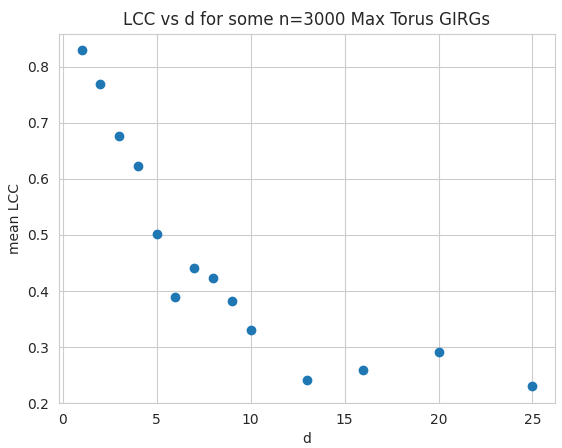
\includegraphics[width=0.8\textwidth]{./figures/LCC_vs_d.png}
    \caption{Increasing the dimension $d$ of a GIRG will decrease the mean LCC, but only up to a $\Theta(1)$ threshold due to the triangle inequality. Each point is one generated GIRG, all other parameters remaining fixed.}
    \label{fig:LCC_vs_d}
\end{figure}



% The first column of copy-weight cube GIRGs in \cref{fig:blasius_framework_table} have much better classification accuracy than the rest, apart from copy-weight Chung-Lu, which serves as the non-geometric comparison point. It would also be interesting to these GIRGs with the configuration model \footnote{Each node is given a set number of "half edges" which gives it a set degree (the degree sequence can be random e.g. power law generated, or given e.g. copied directly from a real graph. Half edges are then joined together at random.)} with copied degrees as the "null hypothesis" against these.

% In notably geometric feature categories like LCC, and diameter GIRGs indeed out perform Chung-Lu.
% Chung-Lu does better on community size statistics; communities could arguably spring from geometry, but GIRGs' uniformly random geometry isn't really designed for this - you could rather imagine a more realistic setup if node locations were taken from a mixture of gaussian distributions (e.g. a university town might have age/occupation clusters of student age vs working age, or academic vs non-academic peoples).


\subsection{Case study of distribution vs mean based classification: closeness centrality}
% \subsubsection{Case study of distribution vs mean accuracy: closeness centrality}
% \addtocounter{subsubsection}{1}
In \cref{fig:blasius_framework_table} which provides feature distributions as input to the SVM classifier, it is disappointing that non copy-weight GIRGs show such poor performance, even on \q{geometric} features like closeness, betweenness and LCC (at least on closeness and betweenness they still recognizably outperform CL, BA and ER). E.g. 2d max torus GIRGs have a misclassification rate of just $1\%$ on \q{n, m, betw} and $2\%$ on \q{n, m, close}, compared to much better $38\%$ and $28\%$ on the mean based classifier equivalents. To explain this large disparity we do a case study on closeness, which happily also assuages some of our concerns.

\cref{fig:real_2d_closeness_mean_scatter} shows that mean closeness aligns very accurately to the real graphs. Nonetheless, due to a consistently lower standard deviation of closeness in the GIRGs and the fact that the standard deviation of closeness in real graphs fits well as a function of number of nodes, the 2d GIRGs are distinguishable from real graphs on this feature set. We hence find the $2\%$ misclassification rate misleadingly low, and the GIRG's realism in closeness somewhat vindicated.

% This analsyis is similar to that done in \cite{blasius2018towards} to explain $0\%$ LCC misclassification rates for hyperbolic graphs when taking into account distribution of features - they found that hyperbolic graphs have consistently too low LCC standard deviation.

\begin{figure}
    \centering
    \begin{subfigure}{0.45\textwidth}
    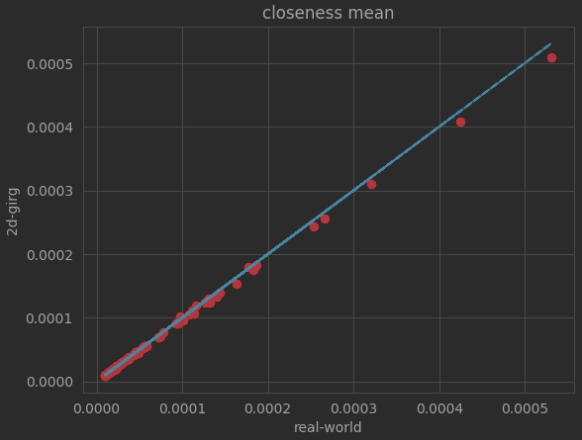
\includegraphics[width=\linewidth]{./figures/real_2d_closeness_mean_scatter.png}
    \caption{2d GIRGs have almost identical mean node closeness to real-world FB graphs; $y=x$ line shown in blue.}
    \label{fig:real_2d_closeness_mean_scatter}
    \end{subfigure}
    \begin{subfigure}{0.45\textwidth}
    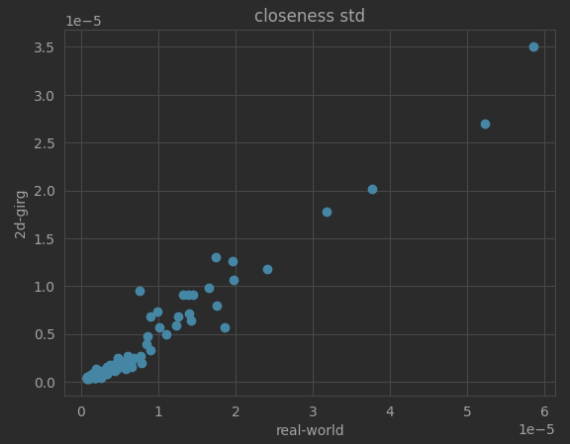
\includegraphics[width= \linewidth]{./figures/real_2d_closeness_std_scatter.png}
    \caption{2d GIRGs have consistently lower standard deviation of node closeness than real-world FB graphs}
    \end{subfigure}

    \parbox[b]{.5\textwidth}{\Large
    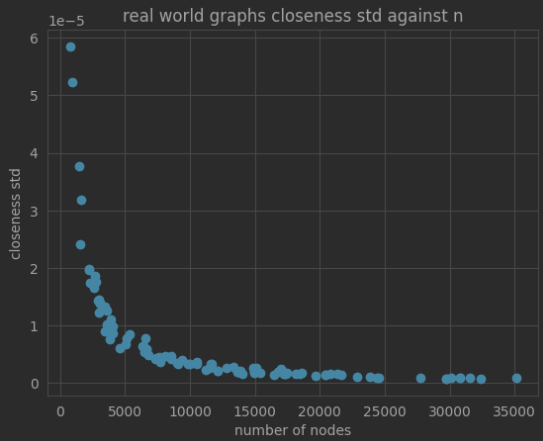
\includegraphics[width=0.9\linewidth]{./figures/real_closeness_std_against_n.png}
    \subcaption{Standard deviation of node closeness in real-world FB graphs fits well as a function of number of nodes}
    }
    \hspace{.05\textwidth}%
    \parbox[b]{.4\textwidth}{%
    \caption{Closeness centrality case study on fit 2d max torus GIRGs against their real counterparts. In plots (a) and (b), each dot is a real / fake graph pair, with the x/y value being the specifid feature's vale for the real/fake graph respectively. In plot (c), each dot is a real graph.}}
    % \begin{subfigure}{0.4\textwidth}
    % 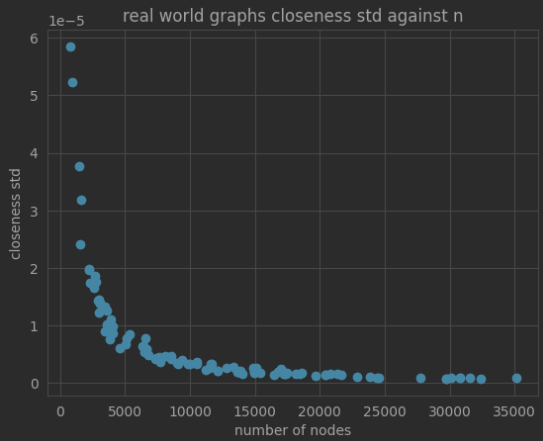
\includegraphics[width=\linewidth]{./figures/real_closeness_std_against_n.png}
    % \caption{standrd deviation of node closeness in real-world FB graphs fits well as a function of number of nodes}
    % \end{subfigure}
    % \caption{Closeness centrality case study on fit 2d max torus GIRGs against their real counterparts. In plots (a) and (b), each dot is a real / fake graph pair, with the x/y value being the specifid feature's vale for the real/fake graph respectively. In plot (c), each dot is a real graph.}
\end{figure}

\subsection{One drawback to the classification realism framework}
Classification accuracy is regrettably a crude metric. One limitation of this framework is that the attainable accuracy is also affected by the level of variance of a feature set across the real graph dataset relative to the fake dataset. GGMs generally end up with their features concentrated in a small subsection of the feature space, so if the real graphs are more spread out, it may be easier to overlap with a portion of their feature data points and attain a low but appreciable misclassification rate. However if the real graphs are less spread out they can miss altogether and get a minuscule misclassifcation rate. See \cref{fig:low_var_high_var_svm_clumps} for an illustration of different scenarios. In this case of closeness, the real graph feature vectors fit quite a precise pattern and hence the GIRG feature vector clump, though just slightly off, has little overlap.


\begin{figure}
    \centering
    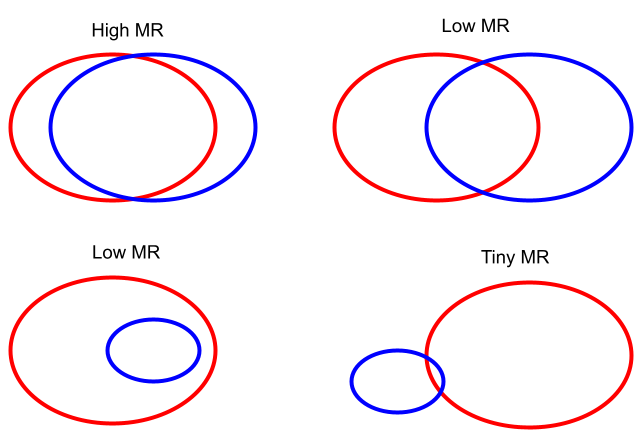
\includegraphics[width=0.9\textwidth]{./figures/VennDiagram.png}
    \caption{Illustration of SVM misclassification rates (MR) given different positions and variance of binary clusters. Red and blue ovals represent roughly gaussian distributed clusters of real and fake data points in a 2 dimensional feature space. An SVM would divide the space so as to maximise classification accuracy. How high accuracy it achieves is directly related to the area/density of overlap between the two clusters.}
    \label{fig:low_var_high_var_svm_clumps}
\end{figure}

% \begin{figure}
%     \centering
%     \begin{subfigure}{0.7\textwidth}
%         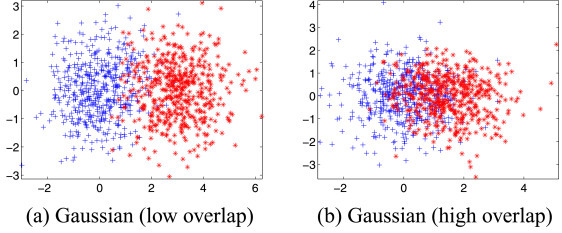
\includegraphics[width=\linewidth]{./figures/high_var_clump_overlaps.png}
%     \end{subfigure}
%     \begin{subfigure}{0.7\textwidth}
%     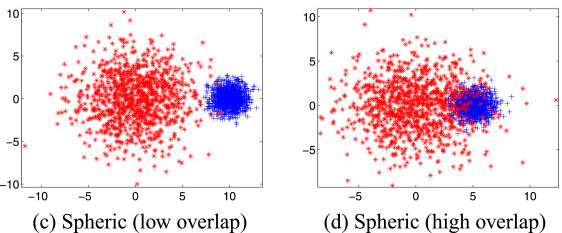
\includegraphics[width=\linewidth]{./figures/low_var_clump_overlaps.png}
%     \end{subfigure}
%     \caption{Plot taken from \cite{kefi2019novel} ("A novel incremental one-class support vector machine based on low variance direction")}
%     \label{fig:low_var_high_var_svm_clumps}
% \end{figure}

% (cube GIRGs having slightly larger diameters - to get from one edge of the cube to the opposite), but does fit our geometric intuition.


% does slightly fit our intuition of their more realistic geometry. Funnily enough Cube GIRGs fit on the dataset have 

% just mean that toroidal GIRGs have too large diameters compared to real graph (cube GIRGs having smaller diameters), but does fit our geometric intuition.

% 2+d min girgs we expect to have very large diameters.

\subsection{SVM Classifier Misclassification Rates Tables}

\begin{sidewaysfigure}
    \centering
    % \begin{subfigure}
    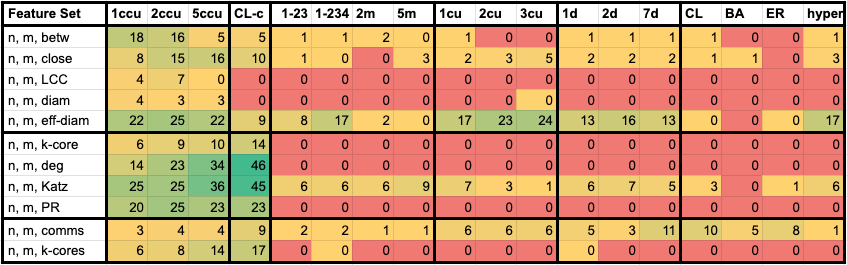
\includegraphics[width=\textwidth]{./figures/Blasius_framework_table.png}
    \caption{\cite{blasius2018towards} GGM realism framework results on Facebook graphs, extended to different GIRG models. Shown here are distribution based features, i.e. including mean, median, lower quartile, upper quartile and standard deviation of node level features.
    % If just one of mean/median is used, accuracies are often lower, sometimes even in $50\%-70\%$. $50\%$ is the best possible validation of a GGM as indistinguishable from real data, and is only achieved for feature set $n, m, LCC \;\text{mean}$ (by GIRGs and not the other none geometric GGMs).
    Some models are missing from the table e.g. 3d-6d GIRGs as their results follow a trend from low to high dimension.
    }
    \label{fig:blasius_framework_table}
    % \end{subfigure}
    \vspace{1em}
    \centering
    % \begin{subfigure}
    \begin{tabular}{|c|c||c|c|}
        \hline
        1-ccu & 1d copy-weight cube GIRG 
        & betw & betweenness centrality
        \\
        1-23 & $1 \lor (2 \land 3)$ mixed min/max GIRG
        & k-core & node k-core number
        \\
        2-min & $1 \lor 2$ 2d min GIRG
        & close & closeness centrality
        \\
        3-cu & 3d cube GIRG
        & LCC & node local clustering coefficient
        \\
        7d & 7d GIRG
        & deg & node degree
        \\
        CL & Chung-Lu
        & Katz & node Katz centrality
        \\
        CL-c & copy-weight Chung-Lu
        & PR & node PageRank
        \\
        BA & Barabasi-Albert
        & comms & community sizes
        \\
        ER & Erdos-Renyi
        & k-cores & k-core sizes
        \\
        hyper & Hyperbolic Random Graph &
        diam & graph diameter
        \\
        && eff-diam & graph effective diameter\\
        \hline
    \end{tabular}
    \caption{Graph Generative Model abbreviations; feature name abbreviations. Used in our results tables}
% \end{subfigure}
\end{sidewaysfigure}

\begin{sidewaysfigure}
    \centering
    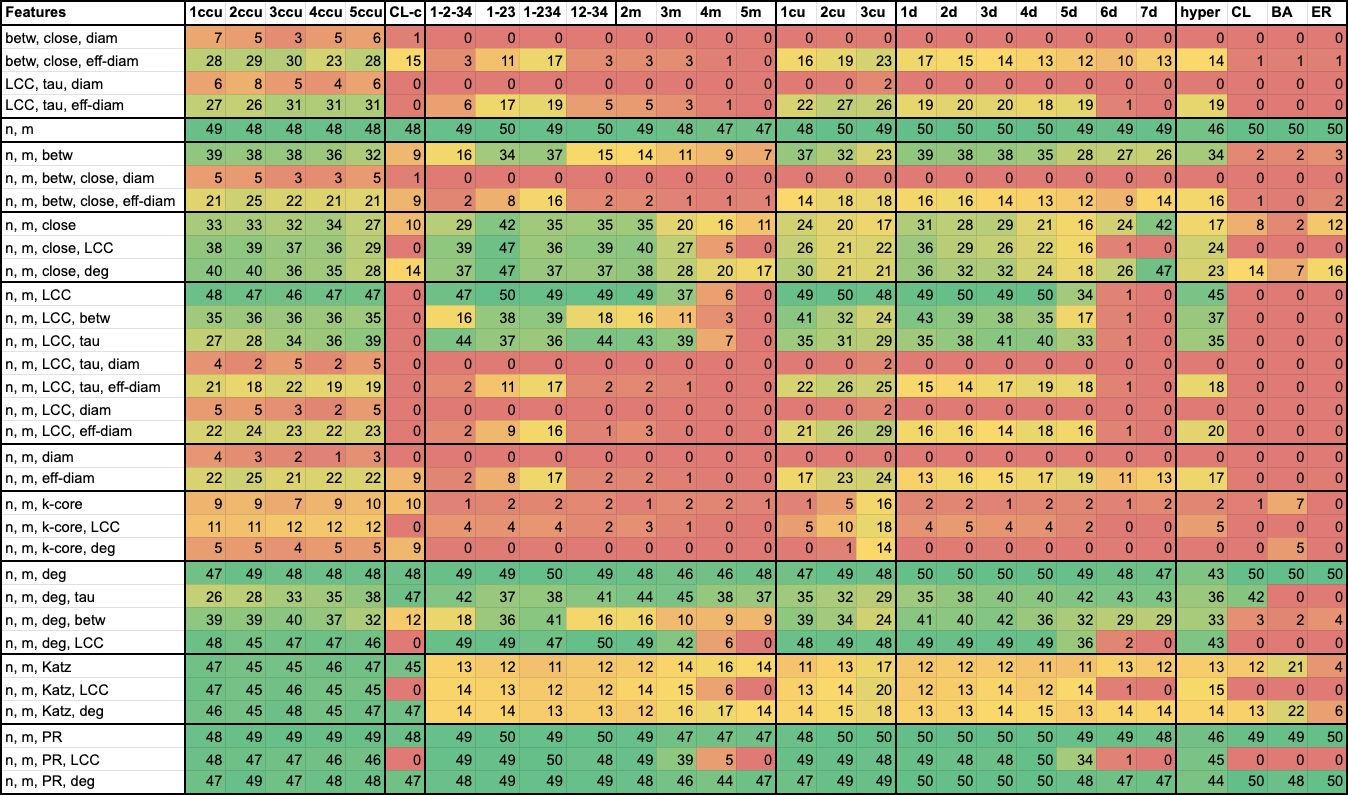
\includegraphics[width=\textwidth]{./figures/blasius_framework_means.png}
    \caption{Blasius Framework classification results based on just mean feature values}
    \label{fig:blasius_framework_means}
\end{sidewaysfigure}


\begin{sidewaysfigure}
    \centering
    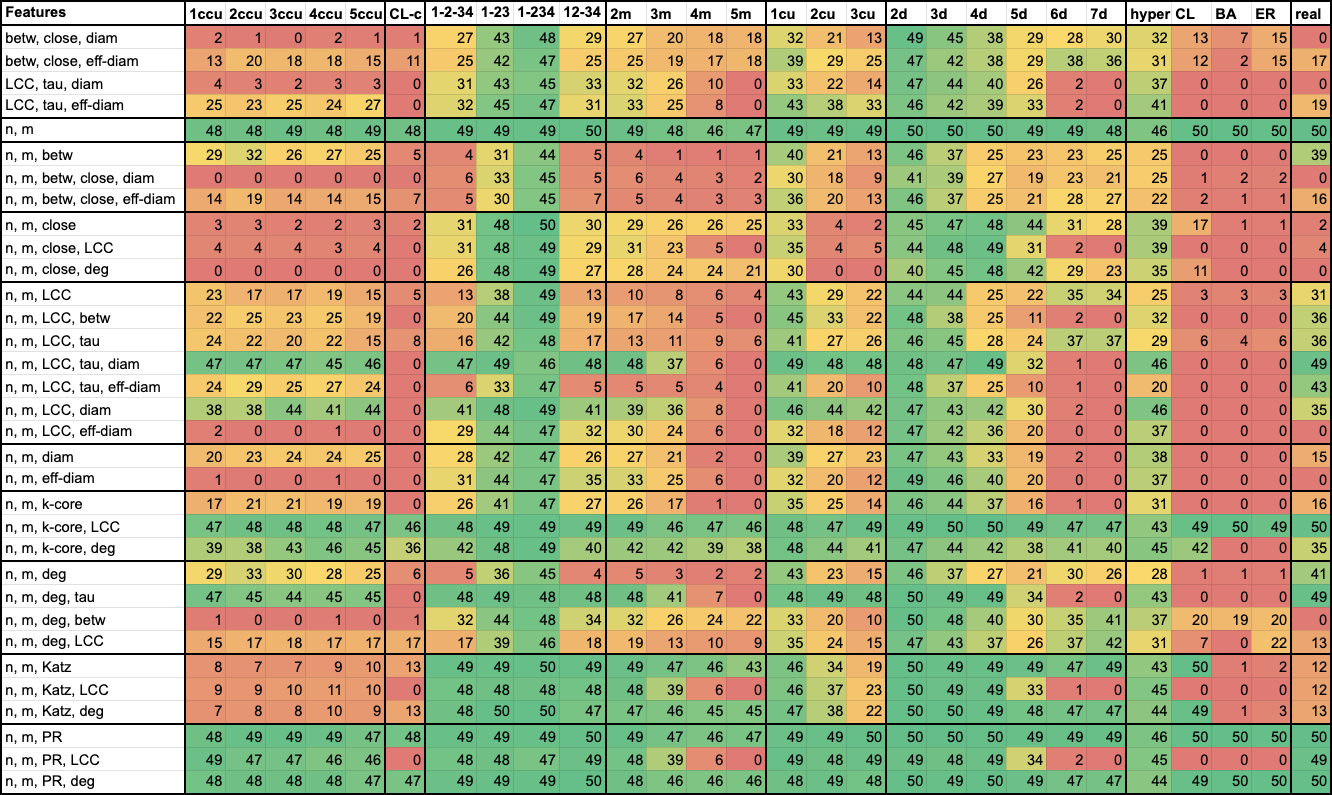
\includegraphics[width=\textwidth]{./figures/blasius_framework_means_1d_base.png}
    \caption{Blasius Framework classification results based on just mean feature values - \q{control} here by classification against the 1d max norm torus GIRG. I.e. all GGMs are still fit to the real graph (so for GIRGs mostly having matching mean node degre and mean LCC), but now the SVM is classifying each GGM against the 1d max norm torus GIRG instead of the real graph.}
    \label{fig:blasius_framework_means_1d_base}
\end{sidewaysfigure}